\cotefile{147}

\scanpage{108}
\mspage{53}
canonique
\[
D_{\deleted{\unsure{p}}d}\longrightarrow X
\]
\margin{On introduit aussi $D_0=X$, (152) et $D_0\longrightarrow X$ l'identité}
qui se factorise d'ailleurs par $D$, et qui est un morphisme d'immersion local, de codim $p$. Pour $D_{\deleted{\unsure{p}}d}$, on a un revêt\textsuperscript{t} étale à $p$ feuillets, noté $\overset{\deleted{\unsure{q}}}{\widetilde D_{\deleted{\unsure{p}}d}}$, \deleted{formé des couples}\inserted{dont la fibre en} un pt $(x,V)$ est \unsure{formée|formé} de l'ens des $\deleted{\unsure{p}}d$ branches $D_{xi}$ de $D$ en $x$ qui contiennent $V$. Donc les \deleted{\unsure{points|couples}} pts de $\widetilde D_{\deleted{\unsure{p}}d}$ correspondent aux triples $(x,V,W)$, où $x$ est un pt de $D$, et $V\subset W$ des germes de ss-multiplicités de $X$ en $x$ attachées à $D$, de codim. respectives $\deleted{\unsure{p}}d$ et $1$. On trouve donc un morphisme canonique
\diagram{\begin{tikzcd}[ampersand replacement=\&, row sep=small]
\widetilde D_{\deleted{\unsure{p}}d}\arrow[r] \& D_1\\
(x,V,W)\arrow[r,mapsto] \& W
\end{tikzcd}}

Plus généralement, si $J$ est un ens. \unsure{fini} ordonné comme ci-dessus, \inserted{muni d'une fonction codim,} on \deleted{\unsure{en}} désigne par $D_J$ la \deleted{\unsure{var.}} multiplicité \deleted{formée}\inserted{dont} les points sont les couples d'un $x\in\deleted{D}\inserted{X}$ \inserted{de codim $d=d(J)$,} et d'un plong\textsuperscript{t} d'ens. ordonnés, compatible \unsure{aux|\deleted{avec}} fonctions codim
\margin{on suppose la fonction codim strictement décr. cf (151)}
\[
(152)\qquad J\mathrel{\overset{\varphi}{\hookrightarrow}}\Delta_x\simeq\mathcal P(I(x))^\circ
\]
\margin{107}

\scanpage{109}
\deleted{On va \deleted{\unsure{désormais|d'ailleurs}} supposer que $J$ a un plus petit élément $e_J$, soit $d(J)=d$ sa codim.}

Alors la multiplicité $D_J$ est lisse, \deleted{de} et le morphisme canonique
\[
(153)\qquad D_J\longrightarrow X
\]
est une imm. \unsure{locale|local} de codim $d$.
Elle se factorise par $D$, sauf dans le cas où $d(I)$\inserted{$=0$ i.e. $I$} est réduit à un seul élément, de codim. nulle, auquel cas $D_J=\deleted{D_0}=X$.

Si $J$ est formé d'un seul élément, de codim $d$, on retrouve $D_d$; S'il est formé de deux éléments, \deleted{le plus} $e_J$ de codim $d$ et $e'$ de codim $1$, on retrouve $\widetilde D_d$.

Si $J$ est de dim totale $d=d(J)$, \unsure{on peut} \deleted{\unsure{retrouver}} \unsure{réconstruire|reconstituer} $D_J$ à l'aide de $D_d$ et de $\widetilde D_d$, via le \unsure{revêtement} principal (torseur sous $\mathfrak S_d$) \unsure{sur} $D_d$ associé à $\widetilde D_d$, soit $\overset{\deleted{\unsure{\sim}}}{D^!_d}$, qui s'identifie aussi à $D_{\mathbf I(d)}$, où $\mathbf I(d)$ l'ens ordonné
\diagram{\begin{tikzcd}[ampersand replacement=\&, column sep=small]
\underset{d}{\bullet}\arrow[r,dash]\&\underset{d-1}{\bullet}\arrow[r,dash]\&\underset{2}{\bullet}\arrow[r,dash]\&\underset{1}{\bullet}\arrow[r,dash]\&\underset{0}{\bullet}
\end{tikzcd}}
(drapeau maximal de codim $d$). En effet, considérons,
\margin{Mais l'expression de $\overset{\deleted{\unsure{\sim}}}{D^!_d}$ comme $D_{I_d}$ ne met pas en évidence les opérations de $\mathfrak S_d$ \unsure{sur} $\widetilde D_d$ — pour ceci; il faut prendre \unsure{plutôt} l'ens ordonné $K_d$, \unsure{ayant} un \deleted{\unsure{élément}} plus petit élément de codim $d$, et $d$ éléments de codim $1$\ldots}
\margin{les \unsure{entiers} sont les \unsure{sommets identifiés par} leur codim.}
\margin{108}

\scanpage{110}
\mspage{54}
l'ensemble fini
\[
\begin{aligned}
(154)\quad H(J)={}&\text{ensemble des plongements d'ens. ordonnés, compatibles avec}\\
&\text{les f codim, de }J\text{ dans }\deleted{\mathcal P([1,n]\cap\mathbb N)}\mathcal P(I_d)^\circ\\
&\text{(où }I_d\overset{\mathrm{def}}=[1,d]\cap\mathbb N\text{)}
\end{aligned}
\]
alors $\mathfrak S_d$ opère à gauche sur $H(J)$, et on a un iso. can. de $D$-multiplicités
\[
(155)\qquad D_J\simeq\overset{\deleted{\unsure{\sim}}}{D^!_d}\mathbin{\wedge}_{(\mathfrak S_d)_{D_d}}H(J).
\]

Soient \deleted{$J$} $(J,\underline{\unsure{c|d}})$ et $(J',\underline{c}')$ deux ens. ordonnés finis munis de fonctions codim, et
\[
(156)\qquad J'\mathrel{\overset{f}{\hookrightarrow}}J\deleted{\unsure{'}}
\]
un plong\textsuperscript{t} d'ens ordonnés, compatible aux fonctions codim, on trouve alors un \deleted{application} morphisme canonique
\[
(157)\qquad D_{J\deleted{\unsure{'}}}\longrightarrow D_{J'},
\]
je me demande \deleted{\unsure{sous forme}}\inserted{en termes} de quelles données suppl. \inserted{(si besoin est)} sur les $(D_d,\overset{\deleted{\unsure{\sim}}}{D^!_d})$ on peut reconstituer cette dépendance fonctorielle de $D_J$ \unsure{p.r.|p.v.} à $J$, via (155). \deleted{Considérons}\inserted{Comme la} \deleted{d'abord le plus petit élément $e_{J'}$ de $e$} dépendance fonctorielle en $J$ pour les \uline{iso}
\margin{109}

\scanpage{111}
est clair sur l'expression 155, \deleted{\unsure{les}} $J'\subset J$, Considérons \deleted{le plus petit}\inserted{un} élément \deleted{$\unsure{e'_J|e_{J'}}$}\inserted{$x$} de $J'$, \inserted{$\ne e_J$} \deleted{qui} est de codim $\delta$ \inserted{($\unsure{\ne|\le}d$)} et considérons \inserted{d'abord} le composé
\diagram{\begin{tikzcd}[ampersand replacement=\&, column sep=large,row sep=small]
\text{(158)}\&D_J\arrow[r]\arrow[dr,draw=none,"{\deleted{\searrow}}" description]\&D_{J'}\arrow[r,"f_x"]\&D_\delta\\
\&\&\deleted{D_{d,\delta}}\arrow[ur,draw=none,"{\deleted{\nearrow\,\unsure{\mathrm{can.}|\mathrm{iso.}}}}" description]\&
\end{tikzcd}}
\margin{\inserted{défini par fonctorialité par l'inclusion $\{x\}\unsure{\hookrightarrow|\subset}J'$}}
on va le mettre en relation avec l'hom.
\[
(159)\qquad D_J\longrightarrow D_{d,\delta}
\]
suivant (où $D_{d,\delta}=D_{\Delta(d,\delta)}$, $\Delta(d,\delta)$ étant le drapeau \deleted{type} de type $d,\delta$, i.e. l'ens. ordonné \deleted{avec} fonction codim
\diagram{\begin{tikzcd}[ampersand replacement=\&, column sep=small]\underset{d}{\bullet}\arrow[r,dash]\&\underset{\delta}{\bullet}\end{tikzcd}}
(\unsure{car|si} $\delta<d$!) \deleted{\unsure{resp.}} $\underset{\deleted{d=\delta}}{\deleted{\bullet}}$
\deleted{(\unsure{car|si|et} $\delta=d$)}, on a, en appliquant (155) au cas de $\inserted{J=}\Delta(d,\delta)$, \deleted{au lieu de} \deleted{\unsure{l'}} l'isom canonique
\[
(160)\qquad D_{d,\delta}\simeq\overset{\deleted{\unsure{\sim}}}{D^!_d}\mathbin{\wedge}_{(\mathfrak S_d)_{D_d}}\mathcal P_\delta(I_{\inserted{d}}\deleted{(d)})
\]
D'autre part, on a (avec la notation (154) pour $H(J)$), \deleted{pour} l'élément $x\in J$ fixé de $J$, \inserted{\unsure{où|un|de codim} $d'=\operatorname{cod}(e')$,} une application
\diagram{\begin{tikzcd}[ampersand replacement=\&, row sep=small]
\text{(161)}\&H(J)\arrow[r]\&\mathcal P_\delta(I_d)\\
\&h\arrow[r,mapsto]\&h(x)
\end{tikzcd}}
\margin{110}

\scanpage{112}
\mspage{55}
compatible avec les opérations de $\mathfrak S_d$, d'où un morphisme
\diagram{\((162)\quad\)
\begin{tikzcd}[ampersand replacement=\&, column sep=large,row sep=small]
D_J\arrow[r,"f_x"]\arrow[d,phantom,"\simeq"{rotate=90,description}]\&D_{d,\delta}\deleted{\unsure{'}}\arrow[d,phantom,"\simeq"{rotate=90,description}]\\
\widetilde D_d\wedge_{\mathfrak S_d}H(J)\&\overset{\deleted{\unsure{\sim}}}{D^!_d}\wedge_{\mathfrak S_d}\mathcal P_\delta(I_d)
\end{tikzcd}}
\deleted{Ceci posé, il} Cette application est décrite entièrement en termes du rev. principal $\widetilde D_d$ de $D_d$, de groupe $\mathfrak S_d$, \inserted{et de $x\in J$.} On a d'autre part, par ``fonctorialité \inserted{en $J$\deleted{\unsure{''}} de $D_J$}'', les \deleted{morphismes}\inserted{diagrammes} commutatifs étendant (158)
\[
\deleted{(\unsure{162})\qquad D_{d,\unsure{d'|\delta}}\longrightarrow D_{d'}}
\]
\deleted{et on a}
\diagram{\((163)\quad\)
\begin{tikzcd}[ampersand replacement=\&]
D_J\arrow[r]\arrow[d]\&D_{J'}\arrow[d,"f_x"]\\
D_{d,\delta}\arrow[r]\&D_\delta
\end{tikzcd},}
où $D_J\unsure{-|\to}D_{d,\delta}$ et $D_{d,\delta}\unsure{-|\to}D_\delta$ sont définis par fonctorialité par les inclusions $\deleted{\unsure{\{e\}}}\{x\}\subset\{x,e\}\subset J$. On \deleted{Cela signifie}\inserted{peut voir aussitôt} que $D_J\unsure{-|\to}D_{d,\delta}$ est décrit par la recette (162), donc le composé (158) est connu quand on connaît les $D_{d,\delta}\longrightarrow D_\delta$
\margin{111}

\scanpage{113}
-- et quand les composés (158) sont connus, on vérifie que les morphismes $D_J\longrightarrow D_{J'}$ sont connus,..

On est donc intéressé plus particulièrement par les hom
\[
(164)\qquad D_{d,\delta}\longrightarrow D_\delta\qquad(d>\delta)
\]
qui jouent le rôle des ``morphismes but'' alors que les $D_{d,\delta}\unsure{\longrightarrow|-}D_d$ jouent le rôle de ``morphismes source'', et $D_{d,\delta}$ le rôle de ``\deleted{\unsure{f}}multiplicité des flèches'' (où mor. d'inclusion) -- entre éléments de sous-multiplicité \inserted{de $X$} associés à $D$.

On a des isom can.
\[
(165)\qquad D_{d,d'}\times_{D_{d'}}D_{d',d''}\simeq D_{d,d',d''}\qquad\text{si }d>d'>d''
\]
et on \deleted{\unsure{en}} déduit de cette description les morphismes canoniques
\diagram{
\((166)\qquad\)
\begin{tikzcd}[ampersand replacement=\&, column sep=large,row sep=small]
\& \& D_d\\
\& D_{d,d'}\arrow[ur]\arrow[dr] \&\\
D_{d,d',d''}\arrow[ur]\arrow[dr,dash] \& \& D_{d'}\\
\& D_{d',d''}\arrow[ur]\arrow[dr] \&\\
\& \& D_{d''}
\end{tikzcd}
}
mais non directement \deleted{$D_{d'}$},
\[
(167)\qquad D_{d,d',d''}\longrightarrow D_{d,d''},
\]
mais on note que
\[
(168)\qquad D_{d,d''}\longrightarrow D_d\times D_{d''}
\]
\margin{112}

\scanpage{114}
\mspage{56}
\margin{ceci marche au moins dans le Contexte des espaces analytiques}
est un mono $\unsure{\hookrightarrow|\leftarrow}$, et (167) est déterminé par la condition que son composé avec (168) est donné par les morphismes
\diagram{\begin{tikzcd}[ampersand replacement=\&, column sep=large,row sep=small]
\& D_d\\
D_{d,d',d''}\arrow[ur]\arrow[dr] \&\\
\& D_{d''}
\end{tikzcd}}
qui figurent dans (\unsure{166}).

\margin{on pourrait l'appeler aussi ``\uline{structure de drapeaux} analytiques''}
Une ``\uline{Structure de déploiement d'intersection normale}'' se définit \inserted{d'abord} comme une structure de ``catégorie \inserted{\deleted{multiplicité}} analytique'' $\mathcal D$, i.e. d'une catégorie dans la catégorie des espaces analytiques
\margin{(d'abord \unsure{$\mathcal E$} dans la cat des \uline{espaces} \unsure{analytiques})}
\diagram{\(\displaystyle
(169)\quad\left\{\begin{array}{ll}
D_* & \text{espace analytique des objets}\\[5pt]
D_{**} & \text{\rule{4cm}{0.3pt}\quad flèches}\\[8pt]
\begin{tikzcd}[ampersand replacement=\&,row sep=small,column sep=small,baseline=(current bounding box.center)]
\& D_{**}\arrow[dl,"\sigma"']\arrow[dr,"b"]\&\\
D_*\&\&D_*
\end{tikzcd}
&\text{morphismes ``source'' et ``but''}\\[8pt]
D_*\longrightarrow D_{**} & \text{morphisme ``\unsure{identique|identité}''}\\[8pt]
\multicolumn{2}{l}{(D_{**},b)\times_{D_*}(D_{**},\sigma)\longrightarrow D_{**}}\\[5pt]
\multicolumn{2}{c}{(u,v)\longmapsto v\circ u}\\[5pt]
\multicolumn{2}{l}{\text{(morphisme ``composition des flèches'')}}
\end{array}\right.
\)}
\deleted{\unsure{tt}} ces données satisfont aux axiomes habituels (associativité, unité\ldots) exprimant que
\margin{113}

\scanpage{115}
pour tt $S$, les \deleted{\unsure{ens}} ``p\textsuperscript{ts} de $S$ à valeur dans $\mathcal D$ (formé de $D_*(S)$, $D_{**}(S)$ etc) est une catégorie. On suppose de plus donnée une fonction ``codimension'' sur $D_*$
\[
(170)\qquad D_*\xrightarrow{c}\mathbb N
\]
\margin{c'est inutile, elle sort des autres structures, cf plus bas\ldots}
ce qui revient à une décomposition
\[
(271)\qquad D_*=\coprod_{d\in\mathbb N}D_d
\]
d'où une décomposition correspondante
\[
(172)\qquad D_{**}=\coprod_{d,d'\in\mathbb N\times\mathbb N}D_{d,d'}
\]
où
\[
(173)\qquad\begin{gathered}
D_{d,d'}=\text{im. inverse de }D_d\times D_{d'}\\
\text{par }D_{*,*}\xrightarrow{(\sigma,b)}D_*\times D_*.
\end{gathered}
\]

On fait les hypothèses suivantes
\diagram{\(\displaystyle
\begin{array}{c@{\quad}l}
\begin{gathered}(174)\text{\begin{tikzpicture}[x=1mm,y=1mm,line width=.35pt,baseline=-.5mm]
\draw (0,.6)..controls (.4,.9) and (.8,-.1)..(1.5,.1);
\end{tikzpicture}}\\[-3pt]
\text{\begin{tikzpicture}[x=1mm,y=1mm,line width=.35pt]
\draw (0,1.4)--(2.8,0);\draw (.5,1.5)--(2.8,0)--(2.5,.8);
\end{tikzpicture}}
\end{gathered}
&\left\{\begin{array}{l}
\text{a) }D_{d,d'}=\phi\text{ si }d'>d\quad\text{(le but est de codim}\\
\hfill\leq\text{ la codim de la source)}\\[8pt]
\text{b) le morphisme ``identité'' }D_*\longrightarrow D_{**}\quad\deleted{\text{\unsure{induit}}}\\
\quad\text{(qui se factorise en }\coprod_{d\in\mathbb N}D_d\longrightarrow\coprod_{d\in\mathbb N}D_{d,d}\text{) induit}\\
\quad\text{des iso}\qquad D_d\simeq D_{d,d}\\
\quad\text{(une flèche dont source et but sont de }=\text{ codim,}\\
\hfill\longrightarrow\text{ une identité)}\\[8pt]
\text{c) Pour }d\in\mathbb N\text{ fixé, le morphisme ``source'' }\deleted{\underset{\unsure{\prod|\coprod}\,\unsure{d'|d}}{D_{d\unsure{,}*}}\xrightarrow{b_*}D_*}
\end{array}\right.
\end{array}\)}
\margin{ce sera conséquence de c) ci-dessous (\unsure{thm prouvé?|trop fort?})}
\margin{114}

\scanpage{116}
\mspage{57}
\margin{(174)\quad $\left\{\rule{0pt}{14em}\right.$}
\diagram{\(\unsure{(}\quad\)\begin{tikzcd}[ampersand replacement=\&, column sep=large,row sep=small]
D_{d,*} \arrow[r,"\sigma_d"] \arrow[d,equal,"\mathrm{def}"'] \& D_d \\
\displaystyle\coprod_{\substack{\deleted{\unsure{d'}}\\d'\in\mathbb N}}D_{d,d'}=\sigma^{-1}(D_d) \&
\end{tikzcd}}
qui fait de $D_{d,*}$ un esp. analytique sur $D_d$, \deleted{\unsure{pondéré par $d'$}} relativement ordonné (par la relation de factorisabilité
\diagram{\begin{tikzcd}[ampersand replacement=\&, column sep=small,row sep=small]
{} \& {} \arrow[dd,dotted] \\
\bullet \arrow[ru] \arrow[rd] \& \\
{} \& {}
\end{tikzcd}}
des flèches de source donnée) \inserted{``pondéré'' par $d'$,} et loc. isomorphe à $\deleted{\unsure{E}}\mathcal P(I_d)^{\deleted{\unsure{0|\circ}}}_{D_d}$ \inserted{avec sa relation d'ordre et la fonction ``cardinal''} (--- le faisceau constant d'ensembles ordonnés simpliciaux $\mathcal P(I_d)^\circ$ ---

Cela redonne donc un rev. $D^!_d$ principal de groupe $\mathfrak S_d$, permettant de reconstituer les $D_{d,d'}$ --- mais pour reconstituer $D$, il faut de plus se donner \deleted{\unsure{les}} au moins les $D_{d,d'}\unsure{\text{---}|\longrightarrow}D_{d'}$, et (c'est plus sûr!) aussi
\[
D_{\unsure{d|d^\circ},d'}\mathbin{\times}_{D_{d'}}D_{d',d''}\unsure{\text{---}|\longrightarrow}D_{\unsure{d|d^\circ},d''}
\]
(la flèche composition), car il n'est pas clair, avec les seules hyp. faites jusqu'à présent, que \unsure{le|les} \unsure{morphisme|morphismes}
\[
D_{d,d''}\unsure{\text{---}|\longrightarrow}D_d\times D_{d''}
\]
sont mono ?, i.e. que ``tt flèches sont déterminées par sa source et par son but''. Mais finalement si, c'est une conséquence de c). Donc
\margin{115}

\scanpage{117}
la structure envisagée peut se décrire par

a) famille d'espaces analytiques $(D_d)_{d\in\mathbb N^{\deleted{\unsure{*}}}}$

b) $\forall\,d\in\mathbb N$, un revêtement principal \inserted{$D^!_d$} de $D_d$, de groupe $\mathfrak S_d$ --- d'où des $D_{d,d'}$ $(0\leq d'\leq d)$

\margin{on aura $D_{d,d}\simeq D_{d,0}\simeq D_d$\par $D_{d,1}$ est le rev. à $d$ feuillets de $D_d$ qui correspond à $D^!_d$.}

c) des morphismes
\diagram{\begin{tikzcd}[ampersand replacement=\&,column sep=large]
D_{d,d'}\arrow[r,dash,"b",to path={-- ([xshift=-1ex]\tikztotarget.west) \tikztonodes -- ++(0,-0.07)}]
\& D_{d'} \& (\text{pour }0\leq d'<\unsure{d^\circ|d''}),
\end{tikzcd}}
et en plus des diagrammes cartésiens

\deleted{avec la condition que les morphismes can. (pour $d\unsure{\geq|>}d'\unsure{\geq|>}d''$)}
\[\deleted{D_{d,d',d''}\overset{\mathrm{def}}{=}D_{d,d'}\mathbin\times_{D_{d'}}D_{d',d''}\longrightarrow D_d\mathbin{\underset{\unsure{?}}{\times}}D_{\unsure{d''}}}\]
\deleted{d) $D_{d,d'}\mathbin\times_{D_{d'}}D^!_{d'}\unsure{\sim|\simeq}$}
\deleted{d) $\unsure{D^!_{d'}|D^!_{d,d'}}$}
\deleted{$\unsure{B_{d,d'}|D_{d,d'}}$}

d)
\diagram{\begin{tikzcd}[ampersand replacement=\&,column sep=large,row sep=large]
\&D^!_{d,d'}\arrow[r,very thick]\arrow[d,"\mathrm{can}"']\arrow[dr,phantom,"\uline{\mathrm{cart}}"]
\&D^!_{d'}\arrow[d,"\mathrm{can}"]\\
(175)\&D_{d,d'}\arrow[r,dash,"b"',to path={-- ([xshift=-1ex]\tikztotarget.west) \tikztonodes -- ++(0,0.07)}]
\&D_{d'}
\end{tikzcd}}

où $D^!_{d,d'}$ est le revêtement $\mathfrak S_{d'}$-principal de
\[D_{d,d'}\simeq D^!_d\mathbin\times_{(\mathfrak S_d)_{D_d}}\mathcal P_{d'}(I_d),\]
associé au $d'$-rev. ``tautologique'' de $D_{d,d'}$; --- ce qui donne, pour $D_{d,d',d''}$ déduit de ce rev. de $D_{d,d'}$ par
\[D_{d,d',d''}\overset{\text{déf}}{=}D^!_{d,d'}\mathbin\wedge_{(\mathfrak S_{d'})_{D_{d,\unsure{d'|d''}}}}\mathcal P_{d''}(I_{d'}),\]

\margin{\uline{NB} $D_{d,d'}$ et $D_{d,d',d''}$ sont déduits directement de $D^!_d$.}
un \deleted{\unsure{rev.}} diagramme cartésien
\diagram{\begin{tikzcd}[ampersand replacement=\&,column sep=large,row sep=large]
\&D_{\unsure{d^\circ|d''},d',d''}\arrow[r]\arrow[d]\arrow[dr,phantom,"\mathrm{cart}"]
\&D_{d',d''}\arrow[d]\\
(176)\&D_{d,d'}\arrow[r]\&D_{d'}
\end{tikzcd}}

\margin{116}

\scanpage{119}
que c'est une \tikz[baseline=(i119.base)]{\node[inner sep=0pt] (i119) {immersion locale};
\path (i119.south west)--(i119.south east) coordinate[pos=.36] (u119a) coordinate[pos=.94] (u119b);
\draw (u119a)--(u119b);} d'espaces \deleted{\illegible{1}} analytiques lisses (ou lisses sur un esp. analytique donné, dans une situation relative\ldots);

\deleted{\inserted{de codimens. $d-d'$}}
\deleted{On doit \unsure{faire|fait} l'hyp. de finité, que}
\deleted{Notons que pour que $D_{d,d'}\unsure{\text{---}|\longrightarrow}D_{d'}$ soit une imm. local, il suffit que}
\[
\deleted{D_{d,0}\unsure{\longrightarrow|\text{---}}D_0\quad\text{et}\quad D_{d',0}\unsure{\longrightarrow|\text{---}}D_0}
\]
% Both repeated maps below belong to the cancelled block; oblique strokes mark the cancellation.
\diagram{\begin{tikzcd}[ampersand replacement=\&,column sep=large,row sep=small,
execute at end picture={
\draw ([xshift=-3mm,yshift=5mm]r119a.north west)--([xshift=5mm,yshift=-3mm]r119e.south east);
\draw ([xshift=-8mm,yshift=8mm]r119c.north west)--([xshift=2mm,yshift=-3mm]r119d.south west);
}]
|[alias=r119a]|D_{d,0}\arrow[r,phantom,"\unsure{\longrightarrow|\text{---}}" description]\arrow[d,phantom,"\simeq"{rotate=90,description}]
\&|[alias=r119b]|D_0,\&\text{et}\&|[alias=r119c]|D_{d',0}\arrow[r,phantom,"\unsure{\longrightarrow|\text{---}}" description]\arrow[d,phantom,"\simeq"{rotate=90,description}]\&|[alias=r119d]|D_0\\
|[alias=r119e]|D_d\&\&\&D_{d'}\&
\end{tikzcd}}
\deleted{le soient, comme on voit en considérant}
% The following whole diagram is cancelled, including its arrows and both region annotations.
\diagram{\begin{tikzcd}[ampersand replacement=\&,column sep=large,row sep=large,
execute at end picture={
\path (c119b.south east)--(c119d.north west) coordinate[pos=.5] (c119comm);
\node[anchor=north,inner sep=1pt] at ([yshift=-2mm]c119comm) {$\unsure{\mathrm{comm.}|\mathrm{can.}|\mathrm{canon.}}$};
\path (c119e.north east)--(c119c.south west) coordinate[pos=.5] (c119cart);
\node[inner sep=1pt] at (c119cart) {$\mathrm{cart}$};
\draw ([xshift=-3mm,yshift=1mm]c119e.north west)--([xshift=4mm,yshift=-3mm]c119b.south east);
\draw ([xshift=-4mm,yshift=1mm]c119f.north west)--([xshift=-4mm,yshift=5mm]c119d.north west);
}]
\&|[alias=c119b]|D_{d,0}\arrow[dr]\&\\
|[alias=c119a]|D_{\unsure{d,d',0}}\arrow[ur]\arrow[r]\arrow[d,"\sim"{rotate=90,swap}]
\&|[alias=c119c]|D_{d',0}\arrow[r]\arrow[d,"\sim"{rotate=90}]\&|[alias=c119d]|D_0\\
|[alias=c119e]|D_{d,d'}\arrow[r,Rightarrow]\&|[alias=c119f]|D_{d'}\&
\end{tikzcd}}

Dans le cas lisse ou \unsure{relativ\textsuperscript{t}} lisse, l'hyp. d'imm. local équivaut d'ailleurs à celle de mono local, qui garde un sens dans tout site.

Notons que pour tt $d$ on a

\diagram{(178)\quad \begin{tikzcd}[ampersand replacement=\&,column sep=large,row sep=large]
D_{d,0}\arrow[d,"\sim"{rotate=90,swap}]\arrow[dr,no head]\&\\
D_d\&D_0\overset{\mathrm{def}}{=}X
\end{tikzcd}}
\margin{$\mathcal D$ est une catég. dans la catégorie $(\mathrm{An})_{D_0}$}
donc les $D_d$ s'envoient tous can\textsuperscript{t}. dans $X=D_0$, et on aura commutativité dans

\diagram{(179)\quad \begin{tikzcd}[ampersand replacement=\&,column sep=large,row sep=large]
D_{d,d'}\arrow[r,no head,"b",to path={(\tikztostart.east)--([xshift=-2mm]\tikztotarget.west)--++(.3mm,-.7mm)\tikztonodes}]\arrow[d,"\sigma"']\&D_{d'}\arrow[d]\\
D_d\arrow[r]\&\deleted{\unsure{D_0}}\inserted{X}
\end{tikzcd}}
\margin{118}

\scanpage{120}
\mspage{59}
où $\sigma$ est un rev. étale donc un iso. local. Donc on voit que si $D_d\unsure{\text{---}|\longrightarrow}D_0$ et $D_{d'}\unsure{\text{---}|\longrightarrow}D_0$ sont des immersions locales (resp. des mono. locaux), il en est de $=$ de $D_{d,d'}\unsure{\text{---}|\longrightarrow}D_{d'}$. De plus, dans le cas lisse, on voit que la codim. de $D_{d,d'}\unsure{\text{---}|\longrightarrow}D_{d'}$ est égale à la diff. des codim de $D_d\unsure{\text{---}|\longrightarrow}D_0$ et $D_{d'}\unsure{\text{---}|\longrightarrow}D_0$. On supposera, bien sûr (dernier axiome ! (?))
\[
(180)\qquad D_d\unsure{\text{---}|\longrightarrow}D_0\quad\text{est de codim }d
\]

\deleted{\unsure{NB|Et}} et plus précisément encore ceci. Soit \deleted{\unsure{(181)}} $x\in D_d$, d'où $I(x)$ de cardinal $d$ (tel qu'on ait
\[
(181)\qquad(D_d^!)_x\simeq\mathcal P(I_x)
\]
)
\deleted{qui} \deleted{considérons les} on a aussi
\[
(182)\qquad\begin{aligned}
I_x&=\text{germes de sections en }x\\
&\qquad\text{du rev. }D_{d,1}\text{ au dessus de }D_1\\
&\simeq(D_{d,1})_x,
\end{aligned}
\]
Considérons alors les composés $(i\in I)$
\diagram{\begin{tikzcd}[ampersand replacement=\&, column sep=large]
D_d\arrow[r,"s_i"]\&D_{d,1}\arrow[r,"\substack{\mathrm{can}\\\unsure{1|4}}"]\&\unsure{D_1|D_d}\deleted{\unsure{=D_d}}\arrow[r]\&X
\end{tikzcd}}
qui sont tous égaux au morph. can. $D_d\xrightarrow{i_d}\deleted{\unsure{D_d}}X$, d'autre part les \deleted{$x_i$} \unsure{images} $x_i$ de $x$ dans $D_1$ pr. les $s_i$.
\margin{119}

\scanpage{121}
définissent des germes de sous-espaces \inserted{$D_x^i$} de $X$ en l'image $a$ de $x$ dans $X$, qui contiennent le germe défini par $(D_d,x)\longrightarrow(X,a)$
Ceci dit, on veut que ce dernier germe soit l'\uline{intersection} des germes $D_x^i$, \inserted{et} q. bien sûr que cette intersection soit transversale.

Cette axiomatique inclut des cas tels que
\figure{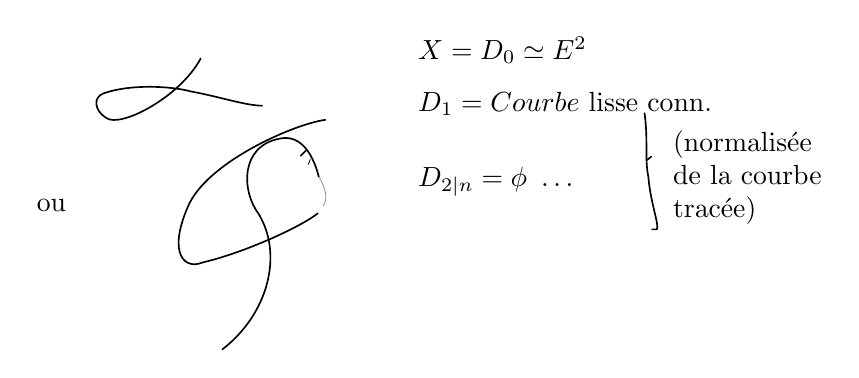
\begin{tikzpicture}[x=.012cm,y=-.012cm,line cap=round,line join=round]
\draw[line width=.6pt] (175,39)
  .. controls (153,80) and (90,113) .. (75,102)
  .. controls (62,94) and (61,80) .. (72,76)
  .. controls (100,66) and (143,68) .. (165,74)
  .. controls (193,79) and (223,89) .. (240,89);
\node at (17,195) {ou};
\draw[line width=.6pt] (307,104)
  .. controls (275,108) and (180,149) .. (161,197)
  .. controls (140,246) and (158,263) .. (177,255)
  .. controls (220,245) and (280,218) .. (299,203);
\draw[black!45,line width=.28pt] (305,195)
  .. controls (310,186) and (307,176) .. (300,164);
\draw[line width=.6pt] (300,164)
  .. controls (293,137) and (279,119) .. (258,124)
  .. controls (217,132) and (218,179) .. (236,203)
  .. controls (263,247) and (246,310) .. (198,347);
\draw[line width=.6pt] (287,136)--(281,142);
\draw[line width=.3pt] (291,146)--(289,151);
\node[anchor=base west] at (395,40) {$X=D_0\simeq\mathbb E^2$};
\node[anchor=base west] at (395,95) {$D_1=\unsure{\text{Courbe}}$ \uline{lisse} conn.};
\node[anchor=base west] at (395,175) {$D_{\unsure{2|n}}=\phi\ \ldots$};
\draw[line width=.6pt] (645,97)
  .. controls (649,126) and (645,145) .. (649,164)
  .. controls (651,191) and (661,216) .. (658,220)--(653,220);
\draw[line width=.6pt] (647,147)--(652,143);
\node[anchor=north west,align=left] at (665,105) {(normalisée\\de la courbe\\tracée)};
\end{tikzpicture}}
qui ne peut être décrit par la donnée d'un diviseur sur $X$, \deleted{lorsqu'on \unsure{en a choisi}}

\deleted{tel diviseur, dans}

L'opération de $\mathfrak S_d$ sur $\mathbb Z^d$ permet de construire sur $D_d$ un système local
\[
(183)\qquad T_d=D_d^!\mathbin\wedge_{(\mathfrak S_d)_{D_d}}(\mathbb Z^d)_{D_d},
\]
\deleted{\unsure{ou}} qui donne naissance à un groupe analytique (et $=$ algébrique) relatif sur $D_d$:
\[
(184)\qquad G_d=T_d\otimes_{\mathbb Z}{\mathbb G_m}_{D_d}\simeq D_d^d\mathbin\wedge_{(\mathfrak S_d)_{D_d}}\mathbb G_m^d
\]
\deleted{Enfin} et $T_d$ s'interprète en termes de $G_d$ comme le syst. local des $\unsure{\Pi_1|\pi_1}$ ou $H_1$ des fibres.
\margin{120}

\scanpage{122}
\mspage{60}
On désigne par $T^!_d$ l'image inverse de $T_d$ sur $D^!_d$, sur lequel $\mathfrak S_d$ opère donc (c'est un \deleted{\unsure{rev}.} syst. local sur $(D^!_d,\mathfrak S_d)\approxeq D_d$). Or sur $D^!_d$ on a les \inserted{$d$} morphismes
\[
(185)\qquad s_i:D^!_d\mathrel{\tikz[baseline=-.5ex,x=1em,y=1ex]{\draw (0,0)--(1.8,0)--(1.84,-.2);}}D_1\qquad(1\leq i\leq d)
\]
permutés par $\mathfrak S_d$, et d'autre part, si $D_1\mathrel{\tikz[baseline=-.5ex,x=1em,y=1ex]{\draw (0,0)--(1.8,0)--(1.84,-.2);}}D_0$ est une immersion \tikz[baseline=(reg122.base)]{\node[inner sep=0pt,outer sep=0pt] (reg122) {régulière};\path (reg122.south west)--(reg122.south east) coordinate[pos=.33] (reg122end);\draw ([xshift=-.2mm]reg122.south west)--(reg122end);} \inserted{de codim 1}, on a \deleted{le \inserted{sur $D_1$} \unsure{faisceau}.} le faisceau \uline{normal} par l'immersion
\[
(186)\qquad L_1\quad\begin{gathered}\text{faisceau inversible}\\\text{canonique sur }D_1\end{gathered}
\]
et on peut considérer sur $D^!_d$ les $d$ faisceaux inv.
\[
(187)\qquad L_{d,i}=s_i^*(L_1)\qquad1\leq i\leq d.
\]
Ils correspondent à des torseurs sous $(\mathbb G_m)_{D_d}$
\[
(188)\qquad\underline L_{d,i}^*=\begin{gathered}{\mathbb G_m}_{D_d}\text{-torseur sur }D_d\text{ associé}\\\text{au faisceau inv. }L_{d,i}\end{gathered}
\]
et on peut considérer
\[
(189)\qquad P^!_d=\prod_{1\leq i\leq d}\underline L_{d,i}^*\qquad\text{torseur sous }\mathbb G_m^d
\]
Comme $\mathfrak S_d$ opérant sur $D^!_d$ permute les \inserted{$s_i$ donc les} $\underline L_{d,i}$ entre eux, il opère sur $P_d$, \deleted{qui} \inserted{de} \deleted{devient} façon compatible avec son opération sur
\margin{121}

\scanpage{123}
\[
(190)\qquad G_d^!\overset{\mathrm{def}}{=}{\mathbb G_m}_{D_d^!}\otimes_{\mathbb Z}T_d^!\simeq\underbrace{{\mathbb G_m^{d}}_{D_d^!}}_{\substack{\text{avec opération de}\\\mathfrak S_d\text{ donnée par}\\\text{permutation des}\\\text{facteurs}}}
\]
et par descente on trouve sur $D_d$ un torseur
\[
(191)\qquad P_d\quad\text{torseur sur }D_d,\text{ de groupe }G_d,
\]
et par suite on a aussi
\[
(192)\qquad T_d\simeq\begin{gathered}\text{\unsure{sys.|syst.} local des }H_1\text{ (ou des }\unsure{\Pi_1|\pi_1}\text{)}\\\text{des fibres de }P_d
\end{gathered}
\]
On considère le groupoïde fondamental $\Pi P_d$ de $P_d$, et \deleted{le groupoïde} \inserted{(quand} $D_d^*$ est défini comme $D_d\setminus(\text{image des }D_{d',d}\mathrel{\tikz[baseline=-0.5ex,x=1em,y=1em]{\draw[line width=.4pt] (0,0)--(.9,0)--(.9,-.13);}}\deleted{\unsure{\text{pour}}}\inserted{D_d}\text{ pour }d'>d,\text{ cf plus bas})$, \unsure{\deleted{\illegible{1}}} plus essentiellement pour la suite,
\[
\Pi(\underbrace{P_d\mid D_d^*}_{\overset{\mathrm{def}}{=}T_d^*})=\Pi P_d^*.
\]
On va considérer la \unsure{variance|variation} des objets précédents $T_d,G_d,\inserted{P_d,P_d^*,}T_d^!,G_d^!,P_d^!,\Pi P_d,\Pi P_d^*$ pour $d$ variable. Considérons donc \inserted{un couple}
\deleted{$d\geq d'$}
\[
d\geq d'\geq0
\]
d'où \deleted{\unsure{avec}}
\diagram{\begin{tikzcd}[ampersand replacement=\&, column sep=large,row sep=large]
\&D_{d,d'}\arrow[dl,"\text{rev. ét}"']\arrow[dr,"\text{imm. }\unsure{\text{local}|\text{locale}}"]\&\\
\unsure{D_d^*|D_d}\&\&D_{d'}
\end{tikzcd}}
\margin{122}

\scanpage{124}
\mspage{61}
considérons les images inverses de $T_d$ et $T_{d'}$ sur $D_{d,d'}$, qu'on va noter
\deleted{${\unsure{T|\mathbb Z}_d}_{D_{d,d'}}$}
\[
(193)\quad\left\{\begin{aligned}
T(d,d')_d&=(T_d)_{D_{d,d'}}&&\begin{gathered}\text{syst. local}\\\text{de rang }d\text{ sur }D_{d,d'}\end{gathered}\\
T(d^{\unsure{*}},d')_{d'}&=(T_{d'})_{D_{d^{\unsure{*}},d'}}&&\begin{gathered}\text{syst. local de}\\\text{rang }d'\text{ sur }D_{d,d'}\end{gathered}
\end{aligned}\right.
\]
on a alors un hom canonique surjectif (dit ``tautologique'')
\[
(194)\qquad T(d,d')_d\mathrel{\tikz[baseline=-.5ex,x=1em,y=1ex]{\draw (0,0)--(1.81,0);\draw (1.8,.15)--(1.82,-.15);}}T(d.d')_{d'}
\]
qui, par image inverse sur $D^!_{d,d'}=D^!_d\mathbin\times_{D_d}D_{d'}$ (cf diagramme can.
\diagram{\begin{tikzcd}[ampersand replacement=\&,column sep=large,row sep=large]
\&\&\mathcal P_{d'}\raisebox{.6ex}{\((I_d)\)}{}_{D^!_d}\simeq D^!_{d,d'}\arrow[dl]\arrow[dr,dash,"\mathfrak S_{d^{\unsure{*}}}",start anchor=south east,to path={-- (\tikztotarget.north west)\tikztonodes -- ([xshift=-1pt,yshift=2.3pt]\tikztotarget.north west)}]\arrow[rr,dashed]\&\&D^!_{d'}\arrow[dd,"\mathfrak S_{d'}"]\\
(195)\&D^!_d\arrow[dr,dash,"\mathfrak S_d"]\&\&D_{d,d'}\arrow[dl,dash,start anchor=south west,to path={-- (\tikztotarget.north east)\tikztonodes -- ([xshift=-1pt,yshift=2.3pt]\tikztotarget.north east)}]\arrow[dr]\&\\
\&\&D_d\&\&D_{d'}
\end{tikzcd}}
s'identifie à l'hom de projection
\[
(196)\qquad\mathbb Z^d\mathrel{\tikz[baseline=-.5ex,x=1em,y=1ex]{\draw (0,0)--(1.81,0);\draw (1.8,.15)--(1.82,-.15);}}\mathbb Z^{d'}
\]
de $\mathbb Z^d$ sur un produit partiel défini par une partie de cardinal $d'$ de l'ens $I_d$ en exposant : $\mathbb Z^d\simeq\mathbb Z^{I_d}$.
\margin{123}

\scanpage{125}
On déduit de (194) un morphisme correspondant (qui est épi lisse)

(197)\quad
\diagram{\begin{tikzcd}[ampersand replacement=\&,column sep=huge,row sep=large]
G(d,d')_d\arrow[r]\arrow[d,equal,"\mathrm{def}"]\&
G(d,d')_{\unsure{d'|d''}}\arrow[d,equal,"\mathrm{def}"]\\
\begin{gathered}G_d\mathbin\times_{D_d}D_{d,d'}\\
\simeq T(d,d')_d\otimes_{\mathbb Z}\mathbb G_m\end{gathered}\&
\begin{gathered}G_{d'}\mathbin\times_{D_{d'}}D_{d,d'}\\
\simeq T(d,d')_{d'}\otimes_{\mathbb Z}\mathbb G_m\end{gathered}
\end{tikzcd}}
et on \unsure{voit|sait} que l'on a un isom. correspondant

(198)\quad
\diagram{\begin{tikzcd}[ampersand replacement=\&,column sep=small,row sep=large]
P(d,d')_{\unsure{d'|d''}}\arrow[d,equal,"\mathrm{def}"]\&
\simeq\&
\underbrace{P(d,d')_d}\arrow[d,equal,"\mathrm{def}"]\&
{}\mathbin\wedge_{\unsure{G_d|G}(d,d')_d}G(d,d')_{d'}\\
P_d\mathbin{\unsure{\otimes|\times}}_{D_d}D_{d,d'}\&\&
P_{d'}\mathbin\times_{D_{d'}}D_{d,d'}\&
\end{tikzcd}}

\inserted{On a des relations de transitivité}
\deleted{Au niveau des groupoïdes fondamentaux, on peut dire que $\Pi P(d,d')_{d'}$}
\inserted{pour les morphismes précédents,}
\deleted{$\unsure{\Pi P(d,d')_d}$}
\unsure{relatifs|relatives} a donnée d'un triple
\[
d\geq d'\geq d''
\]
en se plaçant sur $D(d,d',d'')$, où on a des \deleted{objets} systèmes locaux
\[
(199)\qquad T(d,d',d'')_d,\quad T(d,d',d'')_{d'},\quad T(d,d',d'')_{d''},
\]
des tores correspondants
\[
(200)\qquad G(d,d',d'')_d,\quad G(d,d',d'')_{d'},\quad G(d,d',d'')_{d''}
\]
\margin{124}
